\documentclass[10pt,twocolumn]{icfd2026paper}
\usepackage[dvipdfmx]{graphicx}
\usepackage{ascmac}
\usepackage{amsmath,amssymb}
\usepackage{indentfirst}
\usepackage{newtxtext,newtxmath} %change font 2025/05/09


\newcommand{\bm}[1]{\mbox{\boldmath{${#1}$}}}
\newcommand{\pd}[2]{{\frac{\partial {#1}}{\partial {#2}}}}
\newcommand{\pdd}[2]{{\frac{\partial^2 {#1}}{\partial {#2}^2}}}
\newcommand{\od}[2]{{\frac{{\rm{d}} {#1}}{{\rm{d}} {#2}}}}
\newcommand{\odd}[2]{{\frac{{\rm{d}}^2 {#1}}{{\rm{d}} {#2}^2}}}


%%% Title %%% 
% Please capitalize the first letter of each major word in the title.
\title{Title of Your Paper Here (Initial Capital)}



%%% Names of author(s): Firstame Familyame %%%
% Please underline the presenter using \underline
\author{First Author${}^1$,
\underline{Second Author}${}^1$, Third Author${}^2$ (\underline{Underline for the presenter.})
%%% Email address of the corresponding author %%%
%\footnote for corr. author & e-mail should be placed after the last author
%
\footnote{\normalsize Corresponding author: First Name Family Name}
\footnote{\normalsize {\textit{E-mail address}}:  corresponding\_author@ifs.tohoku.ac.jp}
\\
%%% Affiliation(s) and address %%%
${}^1$ Institute of Fluid Science, Tohoku University \\
2-1-1, Katahira, Aoba-ku, Sendai, Miyagi 980--8577, Japan \\
${}^2$ Affiliation \\
Street, City, State, Zip-code, Country
}
%%%
\abstract{
The abstract should be limited to five lines.
All papers to be published in the proceedings of ICFD must be formatted according to the following instructions. This is a \TeX{} template for preparing your manuscript.
If you prefer MS-Word, a template for MS-Word is also available from the conference website.

This format uses document class, {\tt{icfd2026paper.cls}}. Please use it on your own responsibility.
}
\pagestyle{empty}

\begin{document}

\maketitle
\thispagestyle{empty}

\section{Introduction}

\textbf{The manuscript should be 1-4 A4 pages} and must include the following items:

Title (see the format above)

Name(s) of author(s) and affiliation(s)

Corresponding author's e-mail address (in a footnote)

Abstract

Main text, including table(s) and figure(s)

Conclusions (or Concluding Remarks)

Acknowledgements (if applicable)

References

Appendices (if applicable)\\

\textbf{Please note that all applicants for the Best Presentation Award for Young Researchers, as well as those presenting in a student session, must submit a paper of 2-4 pages.}

\section{Method}
\subsection{Formats}
\subsubsection{Layout}
The main text should be formatted in \textbf{two columns}. Each column must be 8 cm wide and justified. The spacing between the columns must be 1 cm. The left and right margins must be 2 cm, and the top and bottom margins must be 2.5 cm.

\subsubsection{Font}
The manuscript should be prepared in “Times New Roman” (or equivalent).
The font size should be 12 pt for the title and 10 pt for all other text.

\subsection{Title}
The title should be bold and centered.
The author's name should appear below the title and his/her affiliation and address should appear on a separate line immediately below the author's name. 
All of these lines should be centered. \underline{\textbf{Underline the presenter's name.}}




Leave one line between the title and the author's name, between the author and the abstract, and between the abstract and the main text.
All other line spacings should be one line (single spaced).

\subsection{Equations}
Equations are numbered.
The equation number should be aligned right and the same size as used in the text (10 pt).
\begin{eqnarray}
\frac{d \delta \phi (\bm{r}, t)}{dt} = \nabla ^2 [Ds(\delta \phi (\bm{r}, t))\delta \phi (\bm{r}, t)] + \xi (\bm{r}, t).
\end{eqnarray}

\subsection{Table and Figures}
Figures are reduced to fit within the margins of each column.
Symbols and legends should be legible.
Tables and figures should be numbered in the order in which they appear in the text.
Color figures are acceptable.


\begin{table}[h]
\caption{Table captions go above the table, captions that
are two or more lines should be flush left (one line table
captions should be centered), one line space above and
below the caption.}
\begin{center}
 \begin{tabular}{ccc}\hline
 $x$ & $y$ & $z$\\  \hline
 $0.1$ & $15$ & $-1.0$\\
 $0.2$ & $18$ & $-0.1$\\
 $0.3$ & $20$ & $-0.01$\\ \hline
 \end{tabular}
 \end{center}
 \end{table}

\begin{figure}[h]
\begin{center}
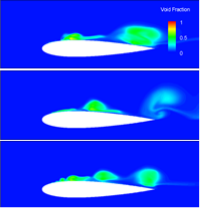
\includegraphics[width=5.5cm,keepaspectratio]{samplefig.png}
\end{center}
\caption{
	Captions with two or more lines should be left-aligned under the figure. Add one blank line above the caption. Single-line captions should be centered beneath the figure.}
\label{fig-disp1}
\vspace{2mm}
\end{figure}


\subsection{References}
References should be numbered in the order of citation and written in the appropriate abbreviated format \cite{HF14, LW13}. Initials should precede the author's surname \cite{refsampleXX}.


\section{Results and Discussion}
Once you have completed your manuscript in the \TeX{} format, create a PDF file.
In \TeX format, submit {\textbf{PDF file only}} from the ICFD web page.
(If using the MS-Word template, submit both Word and PDF files.)
Manuscripts that do not follow these instructions will be returned to the authors.

The proceedings will be available for download from November 9, 2026 to December 31, 2026. The password and URL will be provided to all participants on November 9, 2026.

\section{Concluding Remarks}
The due date of the paper submission is \textbf{July 21, 2026}.

\section*{Acknowledgements (if applicable)}
If this presentation included the results of the Collaborative Research project 2026, please acknowledge the support from the project in the paper with your project code as follows:\\
Part of the work was carried out under the Collaborative Research Project of the Institute of Fluid Science, Tohoku University (Project code: J26****).

\begin{thebibliography}{99}
\bibitem{HF14}
S. Maruyama, T. Yabuki, T. Sato, K. Tsubaki, A. Komiya, M. Watanabe, H. Kawamura, K. Tsukamoto, 
\textit{Deep Sea Res. Part 1}, 58, (2011), 567-547.
\bibitem{LW13}
R.~S.~Loss, S.~B.~Williams,
\textit{Proc. 9th Asia-Pacific Conf. Combust.}, (2013), 809.
\bibitem{refsampleXX}
	Authors, \textit{Proceedings /Book / Journal (abbreviation)}, Volume, (publishing year), page number.
\end{thebibliography}


\end{document}
